\section{Object-centric Development by Example}
\label{sec:PROBLEM}

\subsection{The Game}

We present an example application to give an intuition of object-centric development in Lively. 
The example game, shown in \autoref{fig:game}, features a two-dimensional map where a player character~\textcircled{1} and several \acp{npc} can move about. 
It supports terrains and obstacles, some of which---like water~\textcircled{2} or trees~\textcircled{3}---are impassable. 
The goal of the game is to talk to all of the \ac{npc} on the map~\textcircled{4} and defeat them in debates by choosing the best insults from multiple-choice menus and bringing the morale meter~\textcircled{5} of the opponent down to zero.

\begin{figure}
  \centering
  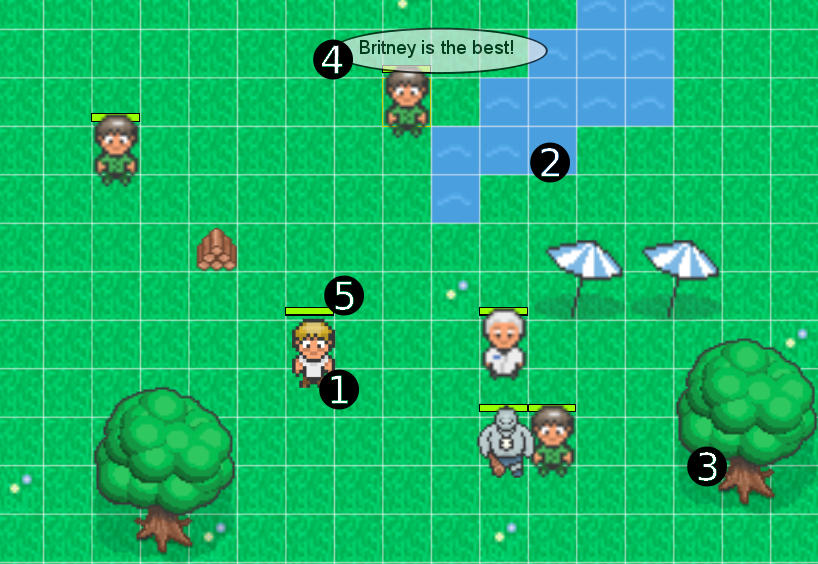
\includegraphics[width=0.7\linewidth]{images/game}
  \caption{\emph{Freedom of Speech} --- The Game}
  \label{fig:game}
\end{figure}

We created this game by adding object-specific behavior to basic components without creating new classes, traits or layers. 
Instead we relied on delegation in two different schemes.
If functionality was required by various different morphs, we implemented it on central components as, for example, the gameboard provides image loading to different objects of our game.
If functionality was required by various similar morphs, however, we composed components out of multiple morphs of which all but one are invisible and capture shared behavior.
For example, the characters are built from copies of the same transparent morph that provides the code for path-finding, user interaction, and debating, while the visible morphs provide appearance and distinct behavior as \emph{costumes}. 
Character morphs load a character picture from the parts bin, and at variation points, like, for example, the phrases they say, they dispatch to their costume morph.

While implementing this game, we observed two shortcomings in Lively's implementation of the object-centric development approach.
First, when we use parts as prototypes and, therefore, copy them to reuse and refine them, we ... 

\subsection{Problems Found}
\begin{itemize}
 \item shared behavior -- work around with costumes pattern
 \begin{itemize}
  \item costumes pattern leads to scattered code, to not browsable code, more objects as necessary
  \item there are objects (base of costume -- tiles, things, player) in PartsBin which are not usable
  \item an objects is artificially splitted into more sub-objects (costume(s) + base)
  \item costume allows grouping of objects, but its hard (a single group might be OK, but multiple groups like moveables, good vs. bad player, hero vs. passive players, ... leads to a high costumes stack)
  \item changing behavior of an object in a group does not change behavior of other objects (copies) in group (excellent-words-to-describe-the-problem-or-... to use: propagation, reload, immediate feedback)
 \end{itemize}

 \item link between editor and edited object
 \begin{itemize}
  \item usual pattern: modules, classes - hierarchies to structure code
  \item tools enables developer to browse along the (usually static) dominant decomposition
  \item lively kernel (with object centric development): morphic scene is dominant composition, because objects are unstructured and only connected through scene graph
  \item browsing through scene graph is hard (halo (there are invisible objects), list selection in object editor (flat list, no hierarchy))
  \item when editing, no scene graph context to object given -- its not possible to locate object or (easily switch to) surrounding objects
 \end{itemize}

\end{itemize}

%%% Local Variables: 
%%% mode: latex
%%% TeX-master: "../paper"
%%% End: 
